% SECTION ====================================================================================
\vspace{-4pt}
\begin{sectionbox}
\section{Heaps}
% ============================================================================================
\subsection{[Max-]Heap}\smallskip
Datenstruktur optimiert zum schnellen Extrahieren von Minimum oder Maximum und Sortieren.\par\smallskip

Binärer Baum mit folgenden Eigenschaften\par
\begin{enumerate}
    \item Vollständig, bis auf die letzte Ebene
    \item Lücken des Baumes in der letzten Ebene höchstens rechts.
    \item \textbf{Heap-Bedingung}:
    \par Max-(Min-)Heap: Schlüssel eines Kindes kleiner (grösser) als der des Elternknotens
\end{enumerate}\smallskip

Baum $\rightarrow$ Array:
\begin{enumerate}
    \item Kinder $(i)=\{2 i, 2 i+1\}$
    \item Elter $(i)=\lfloor i / 2\rfloor$
\end{enumerate}\smallskip

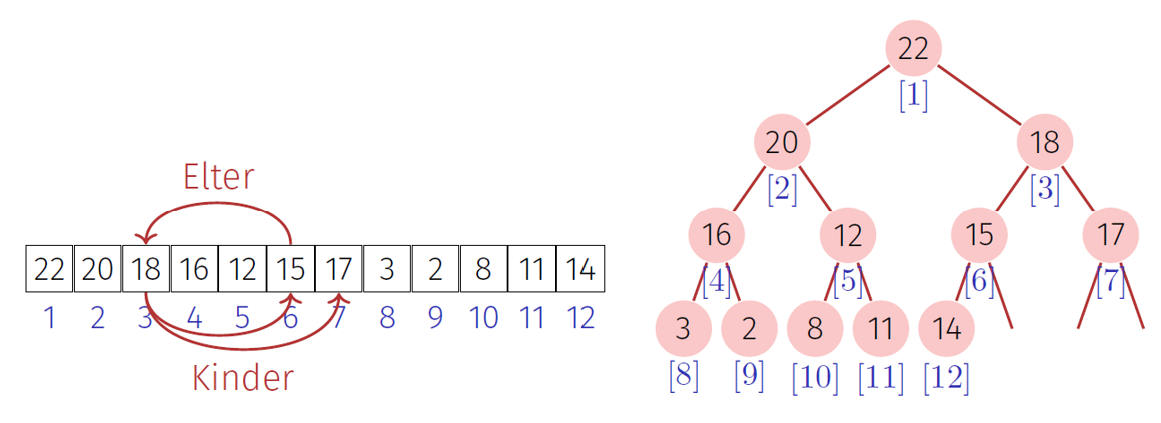
\includegraphics[width = \columnwidth]{../img/heaps.png}\smallskip

\textbf{Höhe eines Heaps}: $H(n)=\left\lceil\log _{2}(n+1)\right\rceil$\par\smallskip

\end{sectionbox}
\vspace{-4pt}
\begin{sectionbox}
\subsection{Heap bauen}\smallskip
\begin{itemize}
    \item Jedes Blatt eines Heaps ist für sich schon ein korrekter Heap. $\rightarrow$ Induktion von unten!
    \item Aufrufe an Versickern: $n/2$. Also Anzahl Vergleiche und Bewegungen $v(n) \in \mathcal{O}(n \cdot \operatorname{log}(n))$.
    \item Versickerpfade sind aber im Mittel viel kürzer: $\mathcal{O}(n)$
\end{itemize}
\end{sectionbox}
\vspace{-4pt}
\begin{sectionbox}
\subsection{Einfügen}\smallskip
\begin{itemize}
    \item Füge neues Element an erste freie Stelle ein.
    \item Stelle Heap Eigenschaft wieder her: \textbf{Sukzessives Aufsteigen}
    \item Anzahl Operationen im worst case: $\mathcal{O}(\operatorname{log}(n))$
\end{itemize}\smallskip
\textbf{Aufsteigen(A,m)}\par
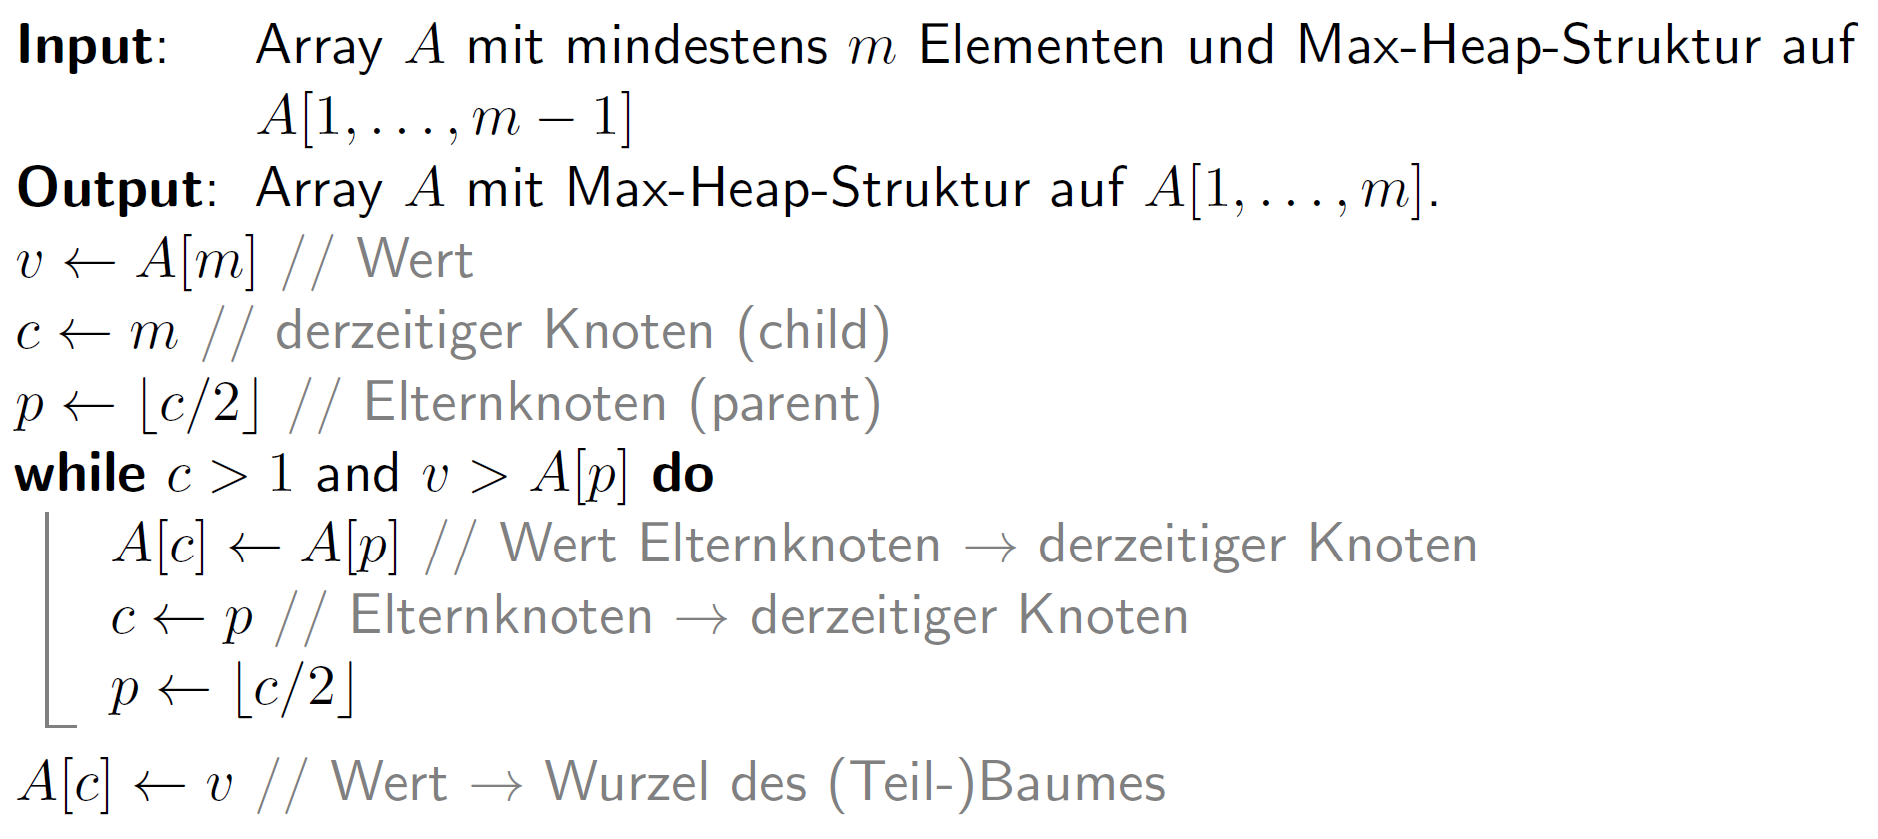
\includegraphics[width = \columnwidth]{../img/Aufsteigen.png}
\end{sectionbox}
\vspace{-4pt}
\begin{sectionbox}
\subsection{Maximum entfernen}\smallskip
\begin{itemize}
    \item Ersetze das Maximum durch das unterste rechte Element.
    \item Stelle Heap Eigenschaft wieder her: \textbf{Sukzessives Absinken} (in Richtung des grösseren Kindes / "Max. aufsteigen lassen")
    \item Anzahl Operationen im worst case: $\mathcal{O}(\operatorname{log}(n))$
\end{itemize}\smallskip
\end{sectionbox}
\vspace{-4pt}
\begin{sectionbox}
\textbf{Versickern(A,i,m)}\par
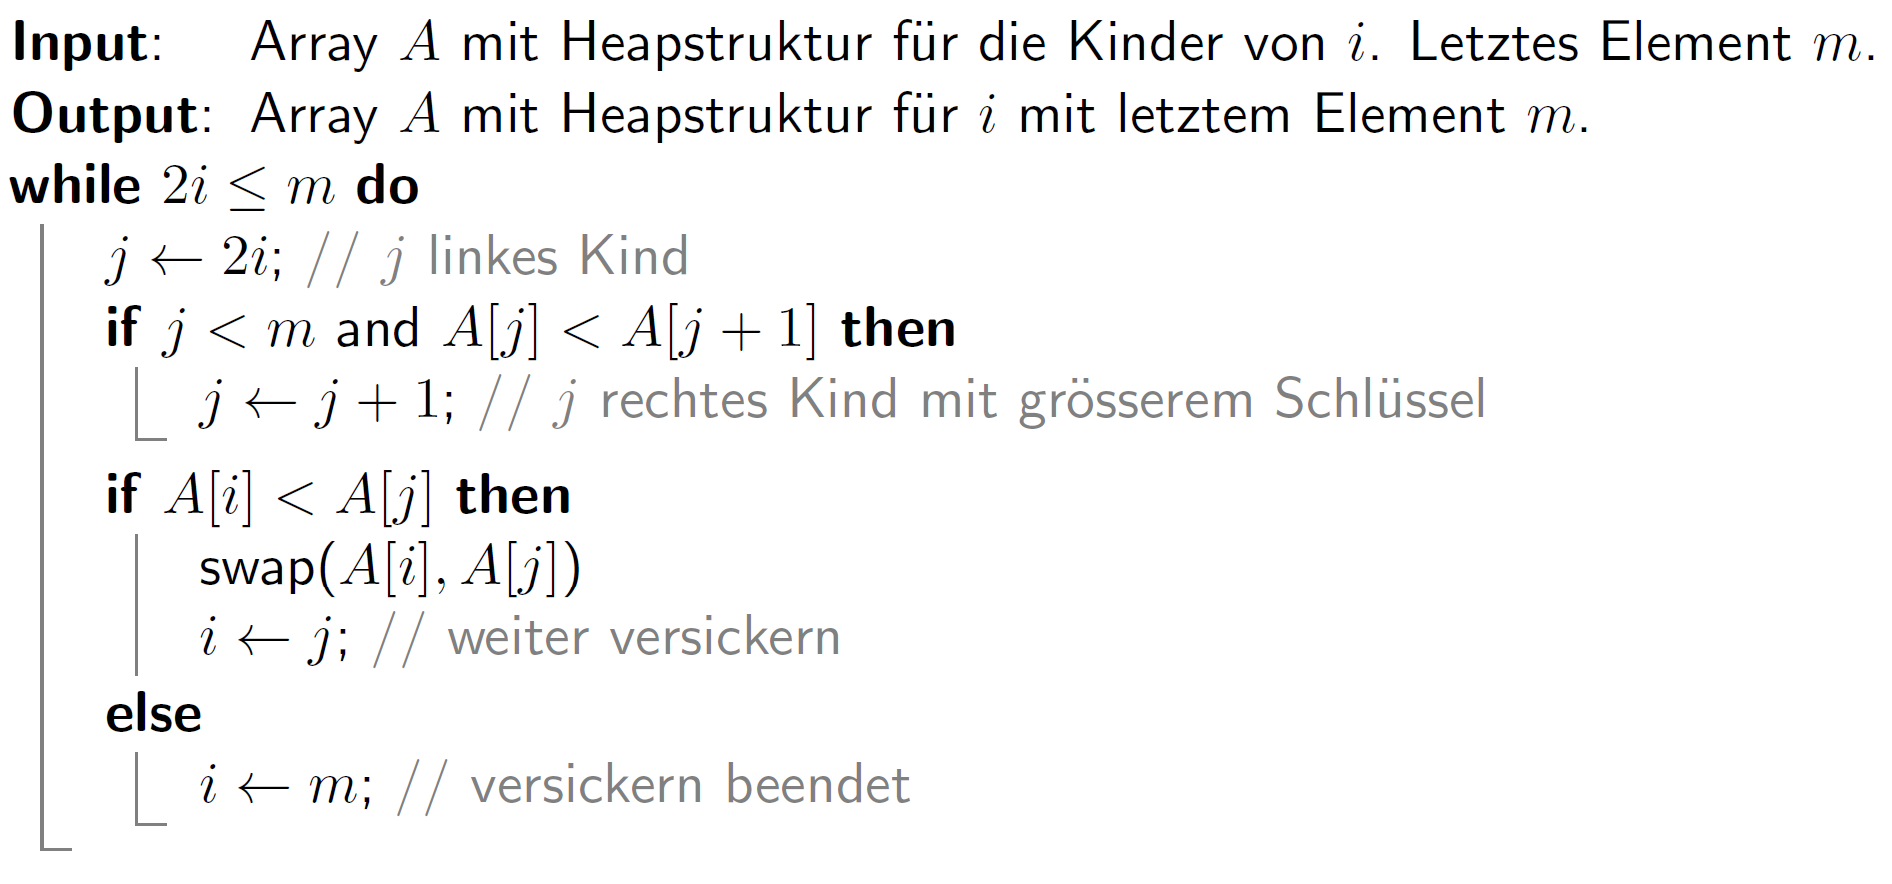
\includegraphics[width = \columnwidth]{../img/Versickern.png}
\end{sectionbox}
\vspace{-4pt}
\begin{sectionbox}
\subsection{Heap sortieren}\smallskip
Worst case: $\mathcal{O}(n \cdot \operatorname{log}(n))$\\
\textbf{HeapSort(A,n)}\par
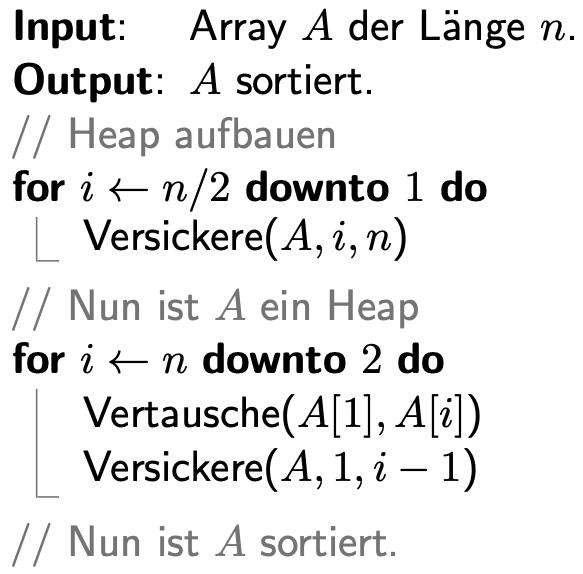
\includegraphics[width = 0.45 \columnwidth]{../img/HeapSort.png}
\end{sectionbox}

